\chapter{Literature review}
\label{LR}

\section{Methods of Modelling Phages and Bacteria}
There are numerous ways to model the interactions between phages and bacteria.
Populations of phages, bacteria, and resources are typically modeled using Ordinary Differential Equations (ODEs) or Delay Differential Equations (DDE). 
DDEs are similar to ODEs, but DDEs incorporate time delays to account for processes that depend not only on the current state but also on past states, such as latency periods in phage infection or delayed bacterial responses to environmental changes.

One way to introduce a delay in an ODE model is to force populations to go through stages, causing a delay in other events. 
For example, in the paper \citet{gengUsingBacterialPopulation2024}, infected bacteria go through $M$ stages of infection, before lysing. 
By decreasing $\tau$ (the latent period) in the model proposed by \citet{gengUsingBacterialPopulation2024}, the throughput of bacteria going from stage $i$ to stage $i+1$ of infection increases, thus seeing a larger rise in phage population. 
All simulations and analyses in this report will use the Golding model, see \Cref{sec:golding_model}. 

Each type of model has its pros and cons.
With the molecular level model, the model is more complex and needs significantly more startup time, simulation time, and is much more complex.
However, more information can be gained from the simulations and can guide research in creating phages for a certain type of bacteria.
The ODE method is simpler to understand and easier to set up, but it can only capture large population dynamics.
Certain assumptions about the community interactions also have to be made, such as the constant washout of the bacteria. 
Each model can be further developed, for example by adding temperature and pH dependence, bacteria releasing nutrients, or if the bacteria concentration is above a certain threshold, the infection rate is lowered to model phages struggling to diffuse through a biofilm. 

\subsection{Generalized Lotka-Volterra Model}
The Lotka-Volterra model, a first-order non-linear differential model, captures the dynamics between predators and prey.
Any population can be modelled as such:
\[ 
    \frac{d{B}_i}{dt} = {B}_i \left(\left(r_i + \sum_{j}^{N} \alpha_{ij}{B}_j \right) - m_i\right)
\]
where $r_i$ is reproduction rate, $\alpha_{ij}$ is the devour rate of $B_i$ on $B_j$. If $\alpha_{ij}$ is negative, then $B_i$ has a negative effect on $B_j$, otherwise $B_i$ has a positive effect on $B_j$. $m_i$ is the removal rate of $B_i$. 
The interactions can be seen in \Cref{fig:lotka_volterra_model}. 

It is possible to add phages into the system by 
 
\subsection{Generalized Consumer-Resource Model}
The generalized Consumer-Resource Model models the growth of a population and resource dynamics between a population of bacteria ${B}_i$ and a resource ${R}_i$. 
\begin{align}
    \frac{d{B}_i}{dt} &= r_i{B}_i \left(\sum_{\alpha} \Delta w_{i \alpha}C_{i \alpha}R_{\alpha}\right) - m_i {B}_i \label{eq:generalized_consumer_resource_model_1}\\
    \frac{dR_{\beta}}{dt} &= -\sum_i C_{i\beta}R_{\beta}{B_i} + \sum_{\alpha, i}D_{\beta\alpha}^{i}C_{i\alpha}R_{\beta}{B}_i \label{eq:generalized_consumer_resource_model_2}\\
    \Delta w_{i\alpha} &= \sum_{\beta}D_{\beta \alpha}^{i}w_{\beta} \nonumber
\end{align}
\Cref{eq:generalized_consumer_resource_model_1} describes the growth of population $B_i$ and \Cref{eq:generalized_consumer_resource_model_2} describes the resource dynamics and metabolism of resource $R_\beta$. 
Resource $R_\alpha$ can become resource $R_\beta$ at rate $R_{\beta \alpha}^{i}$. 
Bacteria $B_i$ reproduces at rate $r_i$ dependent on the concentration of resources $\sum_\alpha C_{i\alpha}$. 
Bacteria die out at rate $m_i$. 
For a visual, see \Cref{fig:consumer_resource_model}

\subsection{Agent-Based Models}
In contrast to Lotka-Volterra and consumer-resource models, ABMs model individual agents and their interactions with other agents and the environment through space and time.
Agents interact with other agents in the vicinity according to some preset rules. 
Non-agent-based entities, such as resources, can diffuse through the environment and are typically modeled using partial differential equations (PDEs) to solve boundary value problems. 
Agents themselves may move between locations with a probability $p$, which can depend on environmental factors or stochastic processes.  
ABMs are used when there is a need to simulate individual entities. 

\begin{align} 
    \label{eq:resource_diffusion}
    \frac{\delta R_\alpha(\left(x, y\right), t)}{\delta t} = \nabla \left[D \left( R_\alpha, \left(x, y\right) \right) \nabla R_\alpha \left(\left(x, y\right), t \right) \right]
\end{align}
\Cref{eq:resource_diffusion} describes the diffusion of resource $R_\alpha$ through space, dependent on the resource concentration $R_\alpha$ at location $(x, y)$. 
The rules for cellular agents follow \Cref{eq:agent_rules}. 
\begin{align} 
    \label{eq:agent_rules}
    \frac{di}{dt} = r_i \left( \sum_\alpha \Delta w_{i\alpha}C_{i\alpha}R_\alpha\right)
\end{align}, 
where $i$ is a bacterial agent. 
\begin{align} 
    \label{eq:agent_consumption_and_conversion}
    \frac{dR_\beta}{dt} &= \sum_i C_{i\beta}R_\beta I + \sum_{\alpha, i}D_{\beta \alpha}^{i} C_{i \alpha} R_\alpha i
\end{align}
\Cref{fig:agent_based_model} shows how the agents interact with other agents in their cell. 

\begin{figure}[h!]
    \centering
    \begin{subfigure}{0.49\linewidth}
        \centering
        \captionsetup{width=1\linewidth}
        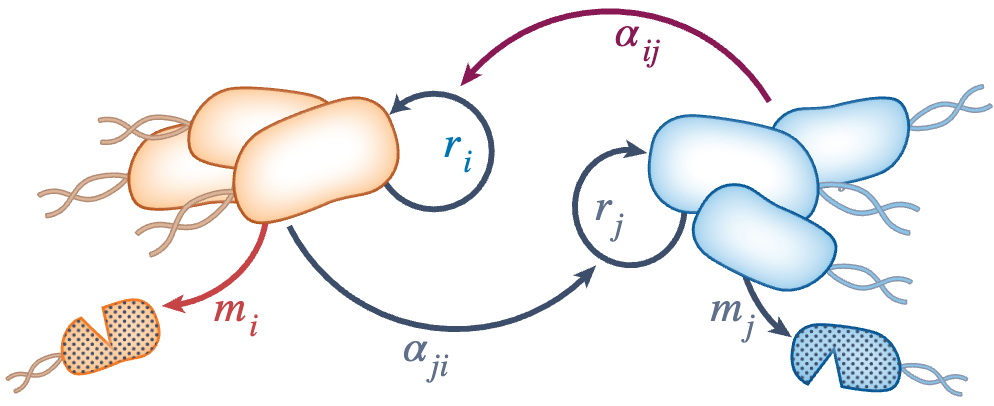
\includegraphics[width=\linewidth]{Figures/lotka_volterra_model.png}
        \caption{
            Lotka-Volterra model.
        }
        \label{fig:lotka_volterra_model}
    \end{subfigure}
    \hfill
    \begin{subfigure}{0.49\linewidth}
        \centering
        \captionsetup{width=1\linewidth}
        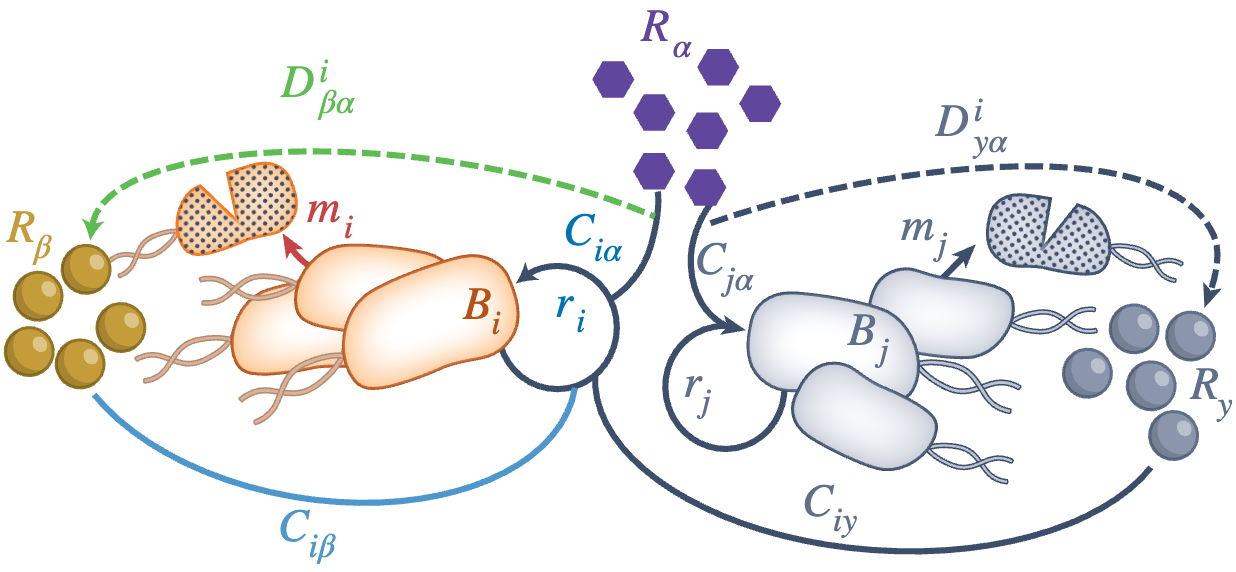
\includegraphics[width=\linewidth]{Figures/consumer_resource_model.png}
        \caption{
            Consumer Resource model.
        }
        \label{fig:consumer_resource_model}
    \end{subfigure}
    \hfill
    \begin{subfigure}{0.49\linewidth}
        \centering
        \captionsetup{width=1\linewidth}
        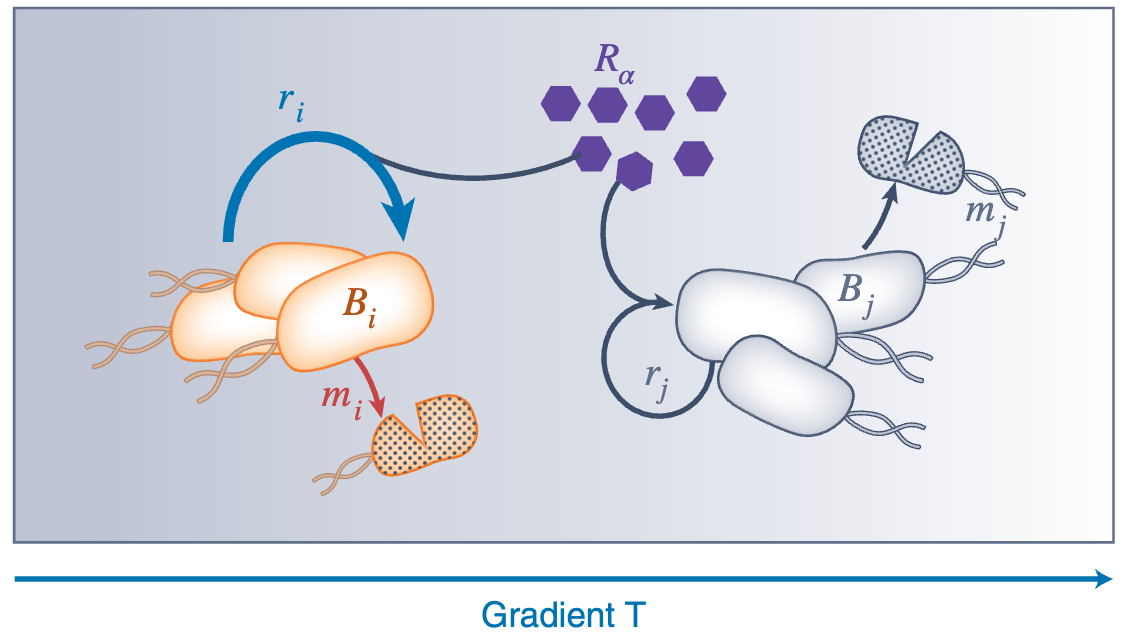
\includegraphics[width=\linewidth]{Figures/trait_based_model.png}
        \caption{
            Trait Based model. 
        }
        \label{fig:trait_based_model}
    \end{subfigure}
    \hfill
    \begin{subfigure}{0.49\linewidth}
        \centering
        \captionsetup{width=1\linewidth}
        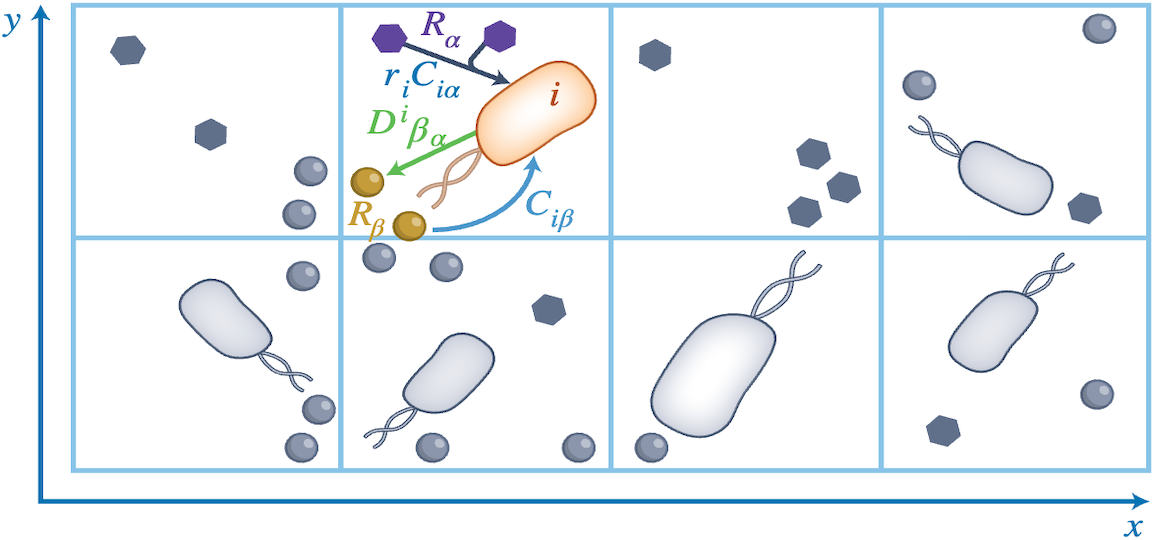
\includegraphics[width=\linewidth]{Figures/agent_based_model.png}
        \caption{
            Agent Based model. 
        }
        \label{fig:agent_based_model}
    \end{subfigure}
    \caption{Different models and how the bacterial entities interact with itself, one another, resources and the environment. All figures sourced from \citet{vandenbergEcologicalModellingApproaches2022}}. 
\end{figure}


\section{Phage Biology}
\subsection{What Are Phages?}
Phages are small bundles of proteins that contain viral DNA. 
Phages are made up of multiple parts built like LEGO to complete the task of infecting a bacterium. 
\Cref{fig:figures:phage_diagram} shows the body parts of a phage. 
The aim of the phage is to find a suitable bacterial host and infect the host with viral DNA. 
The DNA alters the host's metabolic pathways to its benefit and hijacks the cellular replication process to create new copies of the phage. 
Eventually, the cell lyses, releasing the newly created phages into the environment to infect more bacteria. 
\begin{figure}[h!]
    \centering
    \begin{subfigure}{0.25\linewidth}
        \centering
        \captionsetup{width=1\linewidth}
        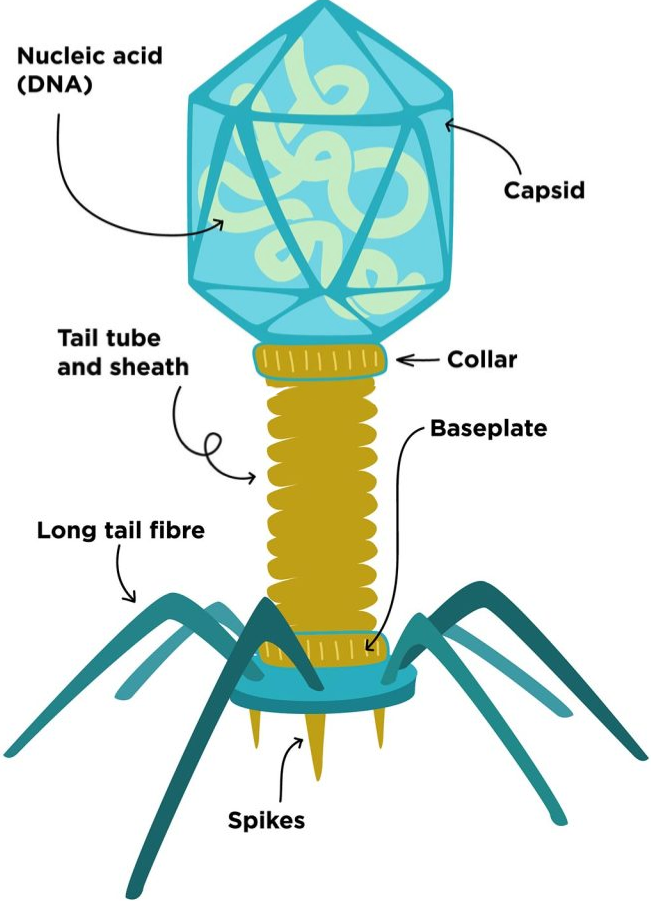
\includegraphics[width=\linewidth]{Figures/phage_diagram.png}
        \caption{
            Phage body structure. 
            % (https://www.newyorker.com/tech/annals-of-technology/phage-killer-viral-dark-matter). 
        }
        \label{fig:figures:phage_diagram}
    \end{subfigure}
    \hfill
    \begin{subfigure}{0.3\linewidth}
        \centering
        \captionsetup{width=1\linewidth}
        \includegraphics[width=\linewidth]{Figures/phage_real.png}
        \caption{
            Phages infecting an \textit{E. coli} bacteria. 
            % (https://www.newyorker.com/tech/annals-of-technology/phage-killer-viral-dark-matter). 
        }
        \label{fig:figures:phage_real}
    \end{subfigure}
    \hfill
    \begin{subfigure}{0.35\linewidth}
        \centering
        \captionsetup{width=1\linewidth}
        \includegraphics[width=\linewidth]{Figures/phage_impression.png}
        \caption{
            Artist representation of phages infecting a bacterium. 
            %(https://www.gettyimages.nl/detail/foto/bacteriophage-virus-attacking-a-bacterium-royalty-free-beeld/1179038792). 
        }
        \label{fig:figures:phage_impression}
    \end{subfigure}
    \caption{Parts of a phage, a real life picture of phages infecting an \textit{E. coli} bacterium, and an artist's impression of phages infecting a bacterium. }
\end{figure}

\subsection{How Does the Phage Cycle Work?}
There are 3 main parts to the phage-bacteria host cycle, the infection stage, the lysogenic cycle, and the lytic cycle. 
In the infection stage, a phage attaches to the surface of a bacteria cell. 
Once injected, the phage-cell pair can go into the lysogenic cycle or into the lytic cycle. 
\Cref{fig:phage_life_cycle} shows a detailed overview of the phage cycle. 
\newline 

In the lysogenic cycle, the phage DNA injects integrates into the genome of the bacteria. 
As the bacteria undergoes cellular replication, the DNA of the phage will be copied with the cell. 
After a set amount of time, the phage DNA can cut itself from the genome and enters the lytic cycle.
\newline 

In the lytic cycle, the phage hijacks the cellular process of the bacteria. 
The phage DNA hijacks the replication, transcription, and replication process of the cell, making more and more copies of phage. 
The phage parts build together to make a full part. 
Eventually the cell wall bursts releasing the phages into the environment ready to infect more bacteria. 

\subsubsection{Infection Stage}
The infection stage is characterized as the searching for a bacterium, detection, and subsequent attachment and injection of DNA into the bacteria. 
\paragraph{Detection and Attachment}
The phage detects the cell via phage receptor binding proteins located at the tip of the phage tail. 
The receptors are tuned to specific receptors found on the surface of the bacteria cell wall. 
Upon detection, conformational alterations in the phage's baseplate occur, causing changes in protein shapes, causing the sheath to contract and inject the viral DNA into the host. 
The successful binding and adsorption depends on the phage binding protein sensitivity, localization,and density of receptors. \cite{stoneUnderstandingExploitingPhage2019}. 
\paragraph{Phage DNA Injection}
The injection is triggered by the recognition between the phage's receptor-binding protein located at the tip of the tail and a specific receptor located on the surface of the bacteria. 
The specificity of recognition is directly related to the specificity of adsorption, which correlates to the structure of receptors located on the host's cell surface \cite{stoneUnderstandingExploitingPhage2019}. 
Once a suitable injection site has been identified, the phage injects the DNA into the cytoplasm of the cell. 
The injected DNA can replicate independently of chromosomes. 

\subsubsection{Lysogenic Cycle}
The lysogenic cycle describes the process in which the viral DNA evades detection, integrates into the cell's DNA, replicates with the cell, and cuts itself from the host's DNA to enter the lytic cycle. 
Prophages are phages that have integrated into the host's DNA. 

\paragraph{Repression of Phage DNA Detection}
Phages need to evade various cellular viral detection methods. 
CBASS triggers effector proteins that cause cell death, preventing phage replication and lysis \cite{banhBacterialCGASSenses2023}. 
Two benefits for the bacteria is that the cell death slows the growth of phages and the dead cells release resources into the environment, allowing other bacteria to recycle the resources and grow \cite{warwick-dugdaleHosthijackingPlanktonicPiracy2019}. 

% CRISPR-Cas is another method that bacteria can use to detect the presence of phage DNA. 
% CRISPR-Cas is an adaptive immune system in bacteria that defends against phages by acquiring foreign DNA sequences (spacers) into its CRISPR array, transcribing them into CRISPR RNAs (crRNAs), and using these crRNAs with Cas proteins to identify and degrade foreign DNA \cite{levyCRISPRAdaptationBiases2015}. 


\paragraph{Phage DNA Integration Into Bacteria DNA}
Phage DNA integrates into the bacterial genome as a prophage. 
This can alter host fitness by modifying metabolic pathways and cellular functions or increasing resistance to other phages, allowing the prophage to persist until conditions favor entry into the lytic cycle \cite{warwick-dugdaleHosthijackingPlanktonicPiracy2019}.

\paragraph{Cellular Replication}
The cell undergoes division multiple times, copying the prophage DNA into the cell copies. 
However prophages are still at risk of being discovered and excised by restriction enzymes \cite{sharpMolecularEvolutionBacteriophages1986}. 
\paragraph{Phage Induction}
Prophages induce (leave) from the bacteria DNA under specific conditions. 
The induction process starts with proteolytic cleavage and displacement of the phage repressor. 

This is typically seen in the lab upon activation of the SOS response following DNA damage \cite{waldorPhageRegulatoryCircuits2005}. 
Cell stressors such as DNA-damaging entities like UV light and antibiotics can jump-start the process to switch to the lytic cycle \cite{stoneUnderstandingExploitingPhage2019, fortierImportanceProphagesEvolution2013}. 

\subsubsection{Lytic Cycle}
The lytic cycle describes the process in which the viral DNA hijacks the DNA replication process, assembles within the cell, and lyses the cell releasing the phages into the environment. 
\paragraph{Hijacking DNA Replication Process}
The phage hijacks the cellular replication process to create the different proteins that make up the phage, like the long tail fiber, tail tube and sheath, and capsid \Cref{fig:figures:phage_diagram}. 
The phage redirects energy and resources from cellular functions towards viral replication \cite{warwick-dugdaleHosthijackingPlanktonicPiracy2019}. 
\paragraph{Assembly of Phage Parts}
Phage parts self-assemble by using various protein-protein and protein-nucleic acid interactions \cite{aksyukBacteriophageAssembly2011}. 
\paragraph{Lysis of the Bacterial Cell}
Many phages produce holin proteins that trigger and degrade the cell wall, releasing the phages and internally stored resources into the environment. 
Holins accumulate in the membrane until a specific time preprogrammed in the protein tells it to destroy the cell wall. 
The protein faces intense evolutionary pressure to control the length of the lytic cycle and ensure lysis at the optimal time \cite{wangHolinsProteinClocks2000}. 

\section{Bacterial Defense Against Phages} 
\label{sec:literaturereview:bacterial_defense_against_phages}
There is a constant battle between phages and bacteria. 
The bacteria don't want to be killed by the phages, so they adapt defenses such as thickening of the cell wall or destroy the viral DNA. 

\subsection{Mutations in Bacterial DNA (Genetic (Co-)Evolution)}
As bacteria cells grow and divide, random point mutations can occur in the DNA. 
These mutations can affect phage defenses, like thickening the cell wall or removing a receptor, making it harder for the phages to detect and infect the cell. 
Mutations can be partially effective if full effectiveness requires multiple steps to achieve. 
Mutations can fail or the mutation brings a cost to the bacteria cell by losing receptors on the cell wall \cite{lenskiTWOSTEPRESISTANCEESCHERICHIA1984}. 

\subsection{Horizontally Transferring DNA}
Bacteria can horizontally transfer DNA to other bacteria on contact. 
A donor cell can donate DNA fragments using a mechanism called the F-factor or plasmid with a pilus. 
The pilus acts as a tunnel between the donor cell and the recipient cell so that DNA can be transferred from the donor cell to the receiver cell. 
This method of sharing DNA can also have the unintended side effect where one bacteria will directly infect another bacteria by transferring phage DNA. 

A phage can accidentally collect a piece of the host's DNA instead of its own DNA during assembly. 
The phage with the now dead hosts DNA can infect the next bacteria, injecting the new bacterium with the dead cell's DNA, horizontally transferring the DNA \cite{tamangHorizontalGeneTransfer2023, kasmanBacteriophages2025}. 
The transferred DNA can include natural phage defenses or significantly alter the DNA of the bacterium that future phages can't detect it anymore. 

\subsection{Phage Inactivation and Decoys}
Bacteria can further protect themselves by producing decoys that the phage will attach to instead of themselves. 
Freshly lysed bacteria may still have biomarkers that attract phages, leading phages to attach to non-viable cells where successful infection cannot occur.
Bacteria can also produce proteolytic enzymes that will damage the proteins found in a phage \cite{tanQuorumSensingDetermines2015}. 
Some bacteria can produce outer membrane vesicles that phages can absorb to, and later detach and float away with the phage \cite{rabinovitchBacterialDebrisEcological2003}. 
It is suspected that the impact of these vesicles acting as a sink is minor \cite{bullPhageBacterialDynamicsSpatial2018}. 

% \subsection{CRISPR-Cas Methods}
% CRISPR is a gene editing tool that cells can use to cut out specified/unwanted parts of a DNA strand. 
% Researchers are commonly using CRISPR to genetically engineer plants and animals to have specific features. 
% Strands of DNA can be selectively added or removed from a DNA strand to achieve a better, more desired DNA strand. 
% CRISPR defenses in the bacteria can detect the unwanted phage DNA and remove the DNA. 

\subsection{Phenotype Resistance}
Not all new phenotypes arise from genetic mutations. 
Resistance can result from phenotypic variation within a genetically identical population, allowing bacteria to express different resistance traits without altering their DNA.
\citet{guptaCombinatorialPhenotypicLandscape2025} found that some \textit{Bacteroides fragilis} bacteria were able to evade phage infection.  
The presence of combinatorial phenotypic states where differential expression of protective mechanisms created rare super-resistant cells capable of withstanding phage attack.
By acting together, these heterogeneously expressed anti-phage defense mechanisms created a phenotypic landscape where distinct protective combinations enabled the survival and re-growth of bacteria expressing these phenotypes without acquiring additional mutations. 

\subsection{Spatial Refuge/Biofilms} 
Usually bacteria and phages coexist in well mixed environments such as the ocean, however some environments offer natural structures for bacteria to hide behind. 
These structures can range from physical structure, like sediment in water to biochemical structures like biofilms, where the phages can't diffuse through the biofilm. 
In large enough quantities, bacteria and other microbial communities create biofilms, a layer of mucus containing various microbes. 
The thick mucus, microbes, and other spatial effects help protect the bacteria in the biofilm from external phages by making it hard for the phages to penetrate and diffuse through the mucus \cite{abedonPhageDelayEnhancing2017}. 
In the case of a lab experiment on an agar plate, bacteria protect one another by making it harder for the phages to diffuse through the system \cite{eriksenGrowingMicrocolonyCan2018}. 

Phage movement is passive, relying on diffusion through the environment or via pressure and temperature gradients \cite{lohrmannInfluenceBacterialSwimming2024}. 
Unlike phages, bacteria possess motility, allowing them to actively move through their environment increasing their chance of survival. 

\section{Phage Counter Defense Against Bacteria}
With some of the defenses that bacteria have developed, phages are always mutating to counter their defenses. 
If phages don't adapt to the ever-changing bacterial defenses, the phages will die out due to their inability to infect and multiply. 
It essentially becomes an arms race, seeing who can out-adapt the other. 
A delicate balance therefore needs to be achieved so that both the bacteria and the phages can coexist. 

\subsection{Genetic Mutations}
Mutations in viral DNA will affect how the phage body parts are designed and built. 
These mutations will affect external phage behavior such as how it detects a bacterium, as well as internal behavior such as evading detection and integrating with the cell's DNA. 
The changes will lead to changes in overall phage fitness, ie the ability for the phage to infect, replicate, and lyse bacteria. 

\subsection{Viral Recombination}
Multiple phages can infect a cell and replicate itself using the cells internal replication process. 
Each phage has its own building blocks. 
If the proteins that build the subparts of each phage have similar chemical properties, they can be swapped between phages \cite{aksyukBacteriophageAssembly2011}. 
This allows for biological diversity to spread throughout a phage population. 
Each phage body part can have unique characteristics such as better attachment rate, larger DNA storage capsule, or better probability of injection. 


\section{Phage Defense Against Phages}
Some phages can employ defenses against other phages from infecting the bacterial cell ensuring the host resources are all for itself. 
The act of preventing a secondary infection from a similar or closely related phage is called superinfection exclusion (SIE) \cite{patelAntiphageDefenceInhibition2024}. 
There are various methods of preventing further infections that are listed below. 

\subsection{Altering Cell Structure}
The prophage can alter the surface receptors of the bacteria, making it harder for other phages to detect the bacteria, reducing the chance of attachment and injection by other phages \cite{bucherPhageMachineSIEence2024}. 

\subsection{Protein Creation}
Other phages like the T4 phage can create proteins like the Spackle protein which inhibits the lysozyme activity used in the process of DNA injection by other phages \cite{bucherPhageMachineSIEence2024, kanamaruStructureFunctionT42020}. 
Some prophages can encode proteins that will interfere with the replication process of other phages. 
For example, the SieA protein encoded by phage P22 blocks infection from other phages \cite{leavittBacteriophageP22SieAmediated2024}. 

Tail Assembly Blocker (TAB) is an anti-phage defense mechanism encoded by a \textit{Pseudomonas aeruginosa} prophage. 
While TAB permits the invading phage to replicate its genome, it inhibits the assembly of the phage tail, thereby preventing the production of infectious virions. 
The prophage that encodes TAB is not affected by this inhibition, as it also expresses a protein that neutralizes TAB's blocking activity. 
Although the host cell still undergoes lysis, no infectious phages are released.

\section{Bacteria and Phages in the Lab}
Researchers around the world are running lab experiments to gain further knowledge of the interactions between phages and bacteria. 
The aim is to better understand how phages work and interact with bacteria at a molecular, host, and population level. 

A researcher might run the experiment in a liquid medium containing water, carbon and nitrogen sources, and other chemicals such as anti-foaming or pH control chemicals. 
This liquid medium, often referred to as broth, allows for the cultivation of bacteria in a well-mixed environment, enabling researchers to monitor bacterial growth and phage infection dynamics over time. 
By adjusting parameters such as resource concentration, temperature, agitation speed, and pH, researchers can simulate different environmental conditions and observe their effects on phage-bacteria interactions. 

Samples can be taken at various time points to measure bacterial density, phage titer, and resource concentration, providing quantitative data for model validation and hypothesis testing. 
If measured frequently enough, the researcher can get an ODE-like curve out, where each datapoint represents the bacteria population level at that time. 
Researchers create a mathematical interpretation of the bacteria growth curve and run curve fitting algorithms to find the model parameters. 
The phage parameters such as latent time and burst size can be found by analyzing the phage one-step growth curve \cite{gengUsingBacterialPopulation2024, mullaExtremeDiversityPhage2024}. 

Commonly used setups include liquids containing phages, bacteria, and resources in a chemostat and batch culture. 
Chemostats allow for continuous addition of resources and removal of waste, maintaining steady-state conditions ideal for studying long-term dynamics.
Bacteria density in clear liquid mediums can be measured optically using light. 
As the bacteria grow and die, the solution will get more cloudy. 
By shining a light through a vial with bacteria growth, the change in light refraction and intensity can be measured. 
A researcher might also be interested in using a mass spectrometer to measure the density of phages and resources at specific time points. 

Petri dishes are another commonly used way to grow bacterial colonies. 
Agar, a jelly-like substance derived from seaweed, is commonly used as a solid growth medium in petri dishes. 
Agar provides a stable surface for bacteria to grow on and form visible colonies. 
Researchers can tailor the nutrients and resources in the medium to support the growth of specific bacterial strains or to test the effects of different environmental conditions. 
When phages are introduced, clear zones called plaques appear where phages have infected and lysed the bacteria, allowing for quantification and observation of phage activity. 
As a cell lyses, it releases phages into the surrounding. 
The phages can diffuse through the system, infecting neighboring cells. 
Phage infection creates clear plaques (2-3 mm) where bacteria are absent. 
See \Cref{fig:phage_petri_dish} for an example.

With petri dishes, it is harder to measure the bacterial growth. 
Bacteria are mixed with phages in a heated liquid agar solution, and poured onto a petri dish. 
It might be possible to wash the bacteria off into a container to measure the optical density (OD), but the results are not always consistent. 
Measuring OD is inaccurate and can only accurately measure up to an OD of 0.1. Even though using a special spectrophotometer allows consistent results, the results are dependent on the medium, the length of travel through the medium, bacteria size and density. 
The device and measurements need to be calibrated to ensure proper results. 
Changing methods to using $\frac{\textit{cells}}{\textit{ml}}$ instead of OD can be used to directly compare results across experiments, labs, and bacteria colonies \cite{miraEstimatingMicrobialPopulation2022}. 

A computer vision algorithm might be able to quantify the change in color on the petri dish, by comparing the photo of the bacterial lawn with a reference photo with no bacteria growth. 
The algorithm could alternatively calculate plaque sizes and determine phage concentration. 
The results are however sensitive to camera settings and external lighting changing the room brightness.  

\begin{figure}[h!]
    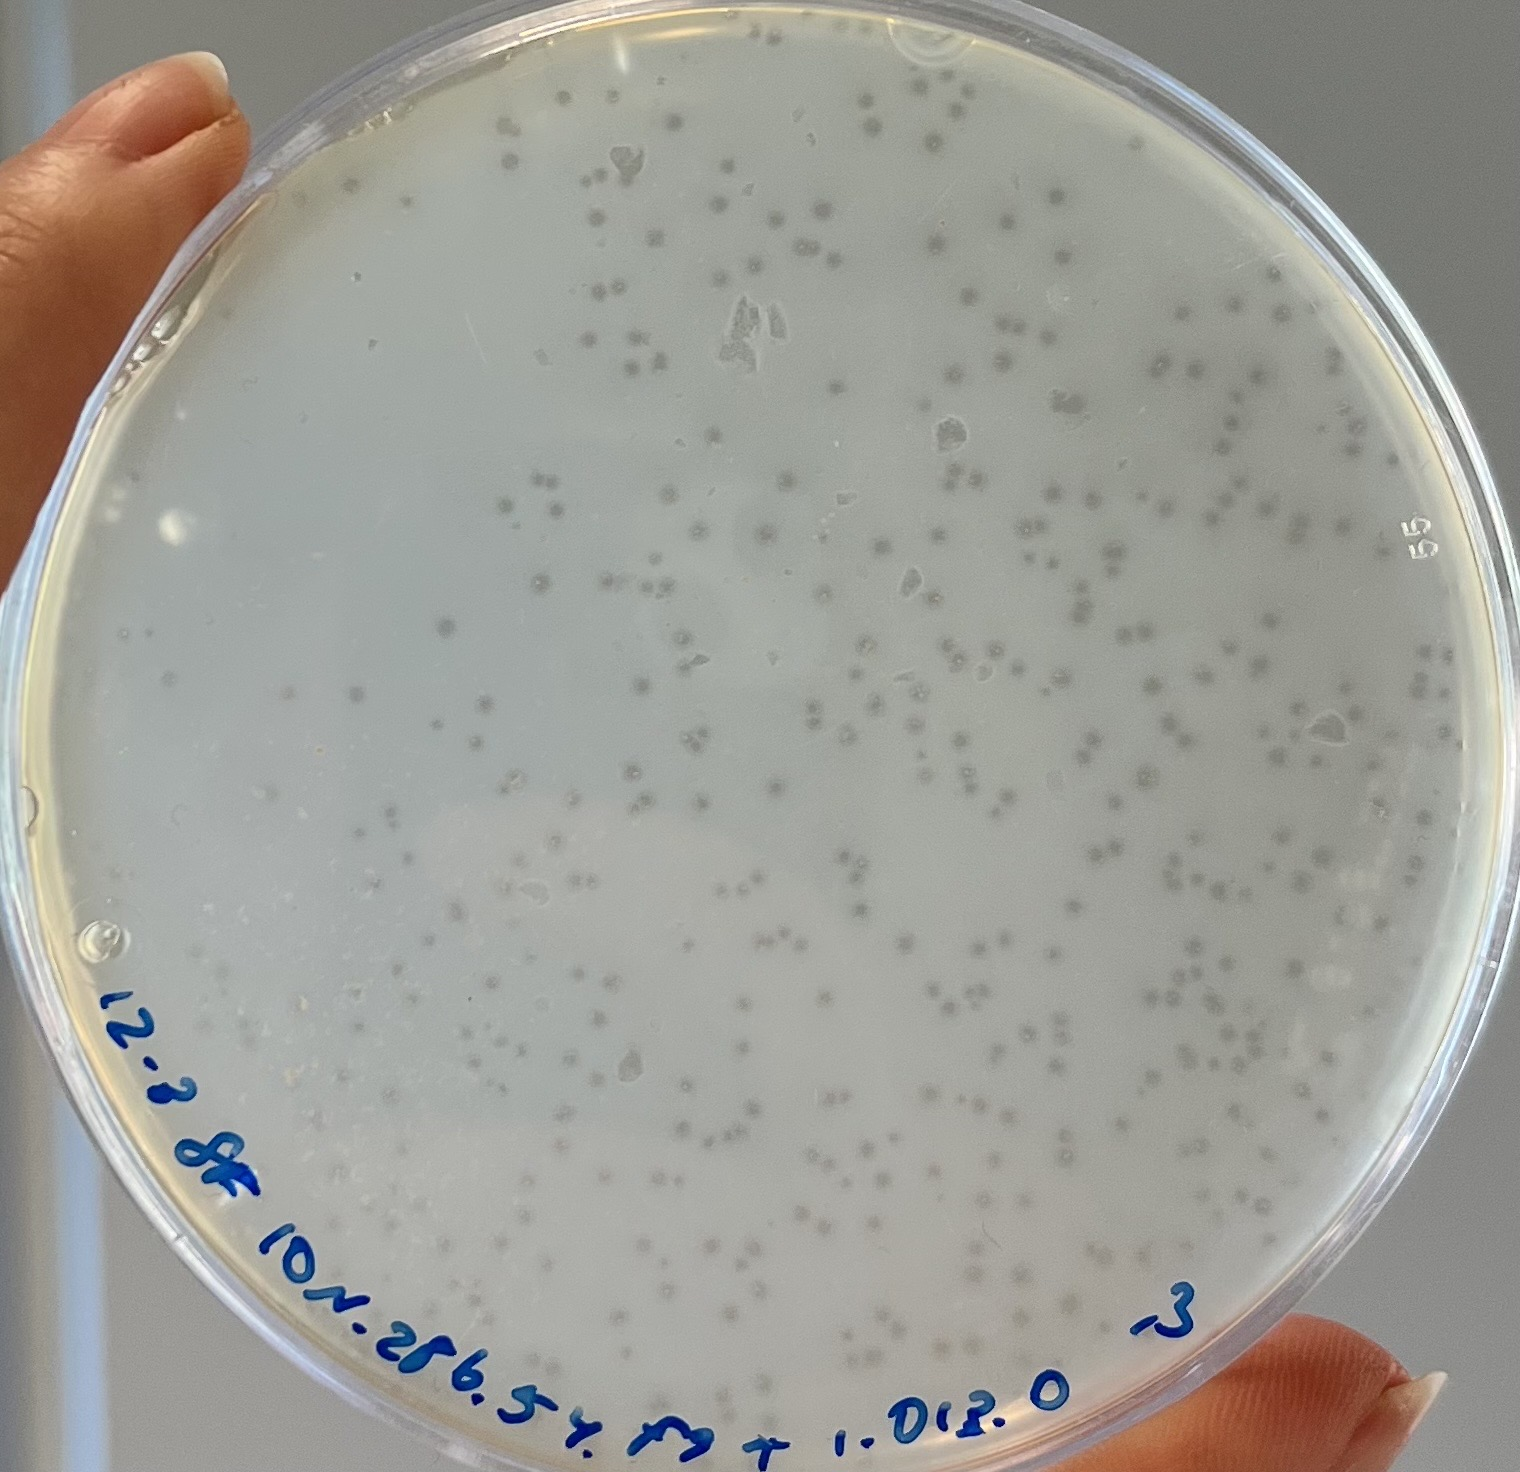
\includegraphics[width=0.5\textwidth]{Figures/phage_petri_dish.jpeg}
    \centering
    \caption{
        Bacteria lawn, the dots on the petri dish show no bacteria growth due to the presence of phages. 
        Photo courtesy of S. Flickinger. 
    }
    \label{fig:phage_petri_dish}
\end{figure}

\subsection{Growth Curves Typically Seen in a Lab}
\label{sec:literaturereview:growth_curves_typically_seen_in_a_lab}

When choosing parameter values it is important to choose parameter values that could realistically be found in real life systems and be replicated in the lab. 
There are various features that a researcher will be looking for in growth curve produced in a lab.
A combination of these features results in an ideal growth curve that replicates real life bacterial growth. 

The idealized dynamics of bacterial populations undergoing phage infection have several phases. First, there is a clear exponential rise in bacteria growth, and can expect to grow 40-100x in the span of a few hours. 
At a certain point in time, the bacteria population start decreasing, almost as fast as they were growing. 

Phage populations also exhibit exponential growth, but with a delay in growth. 
There is initially no growth in phage population. 
After a set amount of time, the phage population will start to grow and peak a few hours after the bacteria population reached its peak. 
If there is no phage death or removal, the phage population will eventually reach a plateau when every bacteria has died. 

\Cref{fig:created:a_good_curve_linear} shows an example of a curve for a $1\times1\times1$ system that would typically be seen in a lab. 
\Cref{fig:created:a_good_curve_logarithmic} is the same plot but with a logarithmic y-axis. 
These specific plots exhibiting a clear growth, peak, delay, and death cycle. 

\begin{figure}[h!]
    \centering
    \begin{subfigure}{1\linewidth}
        \centering
        \captionsetup{width=1\linewidth}
        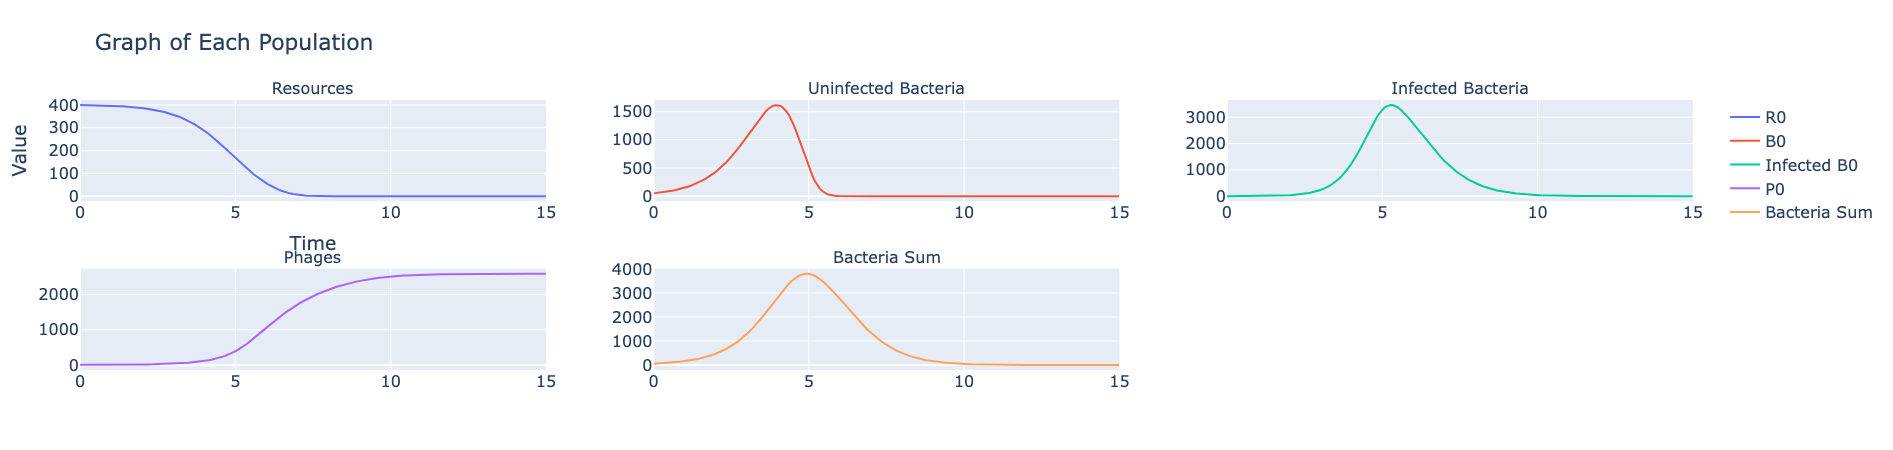
\includegraphics[width=\linewidth]{Plots/Created/a_good_curve_linear.png}
        \caption{
            An example linear y-axis for a curve that researchers aim to replicate. 
        }
        \label{fig:created:a_good_curve_linear}
    \end{subfigure}
    \hfill
    \begin{subfigure}{1\linewidth}
        \centering
        \captionsetup{width=1\linewidth}
        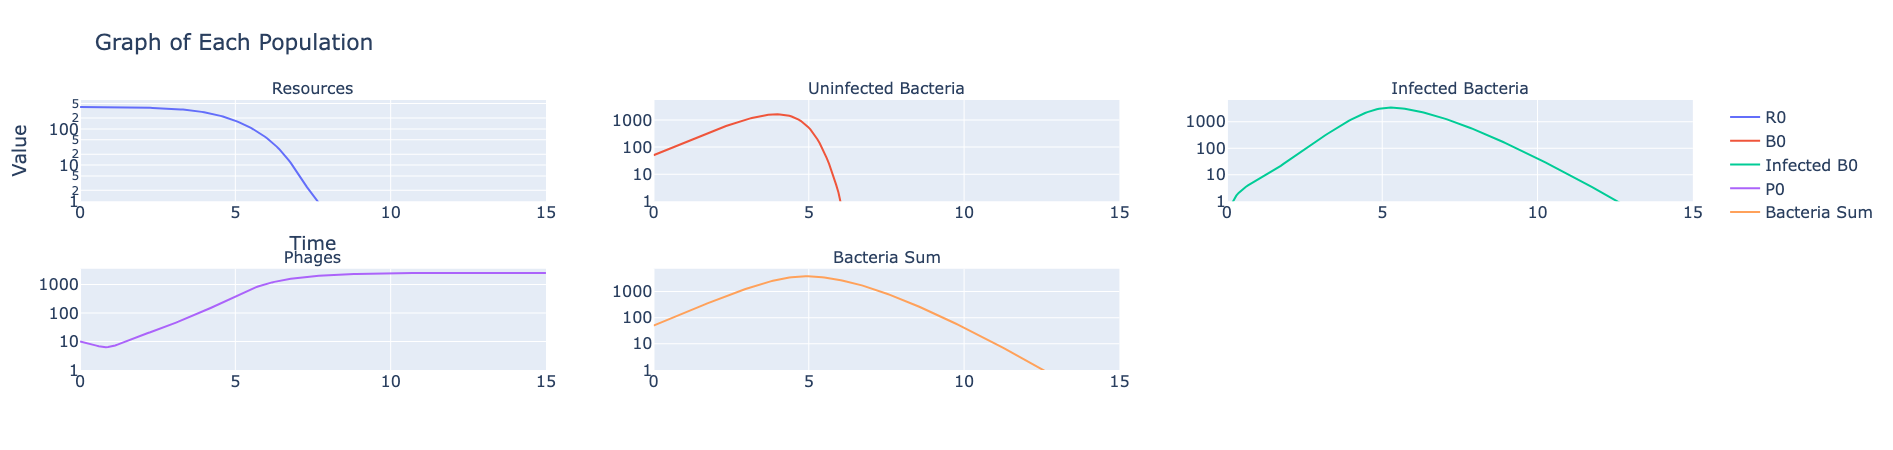
\includegraphics[width=\linewidth]{Plots/Created/a_good_curve_logarithmic.png}
        \caption{
            The equivalent logarithmic y-axis plot for a curve that researchers aim to replicate. 
        }
        \label{fig:created:a_good_curve_logarithmic}
    \end{subfigure}
    \caption{
        Growth population of a $1\times1\times1$ system. 
        The log plot allows to see behavior happening at values approaching and to plot data on a logarithmic scale. 
        The parameters used for this plot can be found in \Cref{tab:appendixE:a_good_curve}. 
    }
    \label{fig:created:a_good_curve}
\end{figure}

\section{Software Mathematically Modelling Phages, Bacteria, and Resources}
Some software programs modelling phage-bacteria-resource interactions already exists. 
\subsection{Cocktail}
\citet{nilssonCocktailComputerProgram2022} developed Cocktail to model phage-bacteria-resource kinetics in a chemostat. 
The model assumes there is one bacteria strain that can be infected by phage A and phage B, and by both phages at the same time, phage AB. 
The model models bacterial resistance to phage A, B, and AB. 
The user can control the parameter values such as resistance rate to A, B, and AB, resource concentration and outflow, and phage adsorption rate. 
The user can also control model settings, such as if the model is deterministic or stochastic, and the step size \cite{nilssonCocktailComputerProgram2022}. 
Four sample output plots are shown in \Cref{fig:sourced:cocktail_plot}. 

\subsection{PhageDyn}
PhageDyn is a Java applet that models phage dynamics in multi-reactor industrial wastewater treatment plant models. 
PhageDyn interacts with existing GPS-X \cite{AdvancedWastewaterModelling} files to incorporate phage dynamics into models of industrial wastewater treatment plants \cite{krysiak-baltynSimulationPhageDynamics2017}. 
\citet{krysiak-baltynSimulationPhageDynamics2017} developed PhageDyn to determine how phages can reduce foaming caused by bacteria in wastewater treatment plants, another real life application of phages \cite{heardEffectFilamentousBacteria2008}. 
PhageDyn does not simulate phage dynamics on its own but rather manipulates existing files in GPS-X in order to incorporate phage dynamics in wastewater treatment plant models. 
\Cref{fig:sourced:phagedyn_plot} shows the output that PhageDyn provides. 

\subsection{Cocktail and PhageDyn Limitations}
\label{sec:literature:cocktail_and_phagedyn_limitations}
There are limitations to Cocktail and PhageDyn. 
Cocktail can model up to a $2\times 1 \times 1$ system, and is designed to model a chemostat. 
Chemostats receive a constant influx of new resources and a constant removal of medium from the chemostat. 
Cocktail's model can not be easily adapted to other models. 
The ODE model accepts inputs from a hardcoded GUI frontend. 
So any changes to the frontend or to the ODE model will require changes to the ODE model and the frontend to accept the new inputs and outputs. 
The code for Cocktail is open source, so adding new buttons and changing the model should not pose a significant challenge, but still an undertaking. 

PhageDyn works with GPS-X, a very niche wastewater treatment modelling software. 
PhageDyn is programmed for a very specific task with no flexibility in changing the model or inputs. 
PhageDyn assumes biomass, instead of individual bacteria populations. 
However, PhageDyn is no longer available for download.

\begin{figure}
    \centering
    \begin{subfigure}{0.49\linewidth}
        \centering
        \captionsetup{width=1\linewidth}
        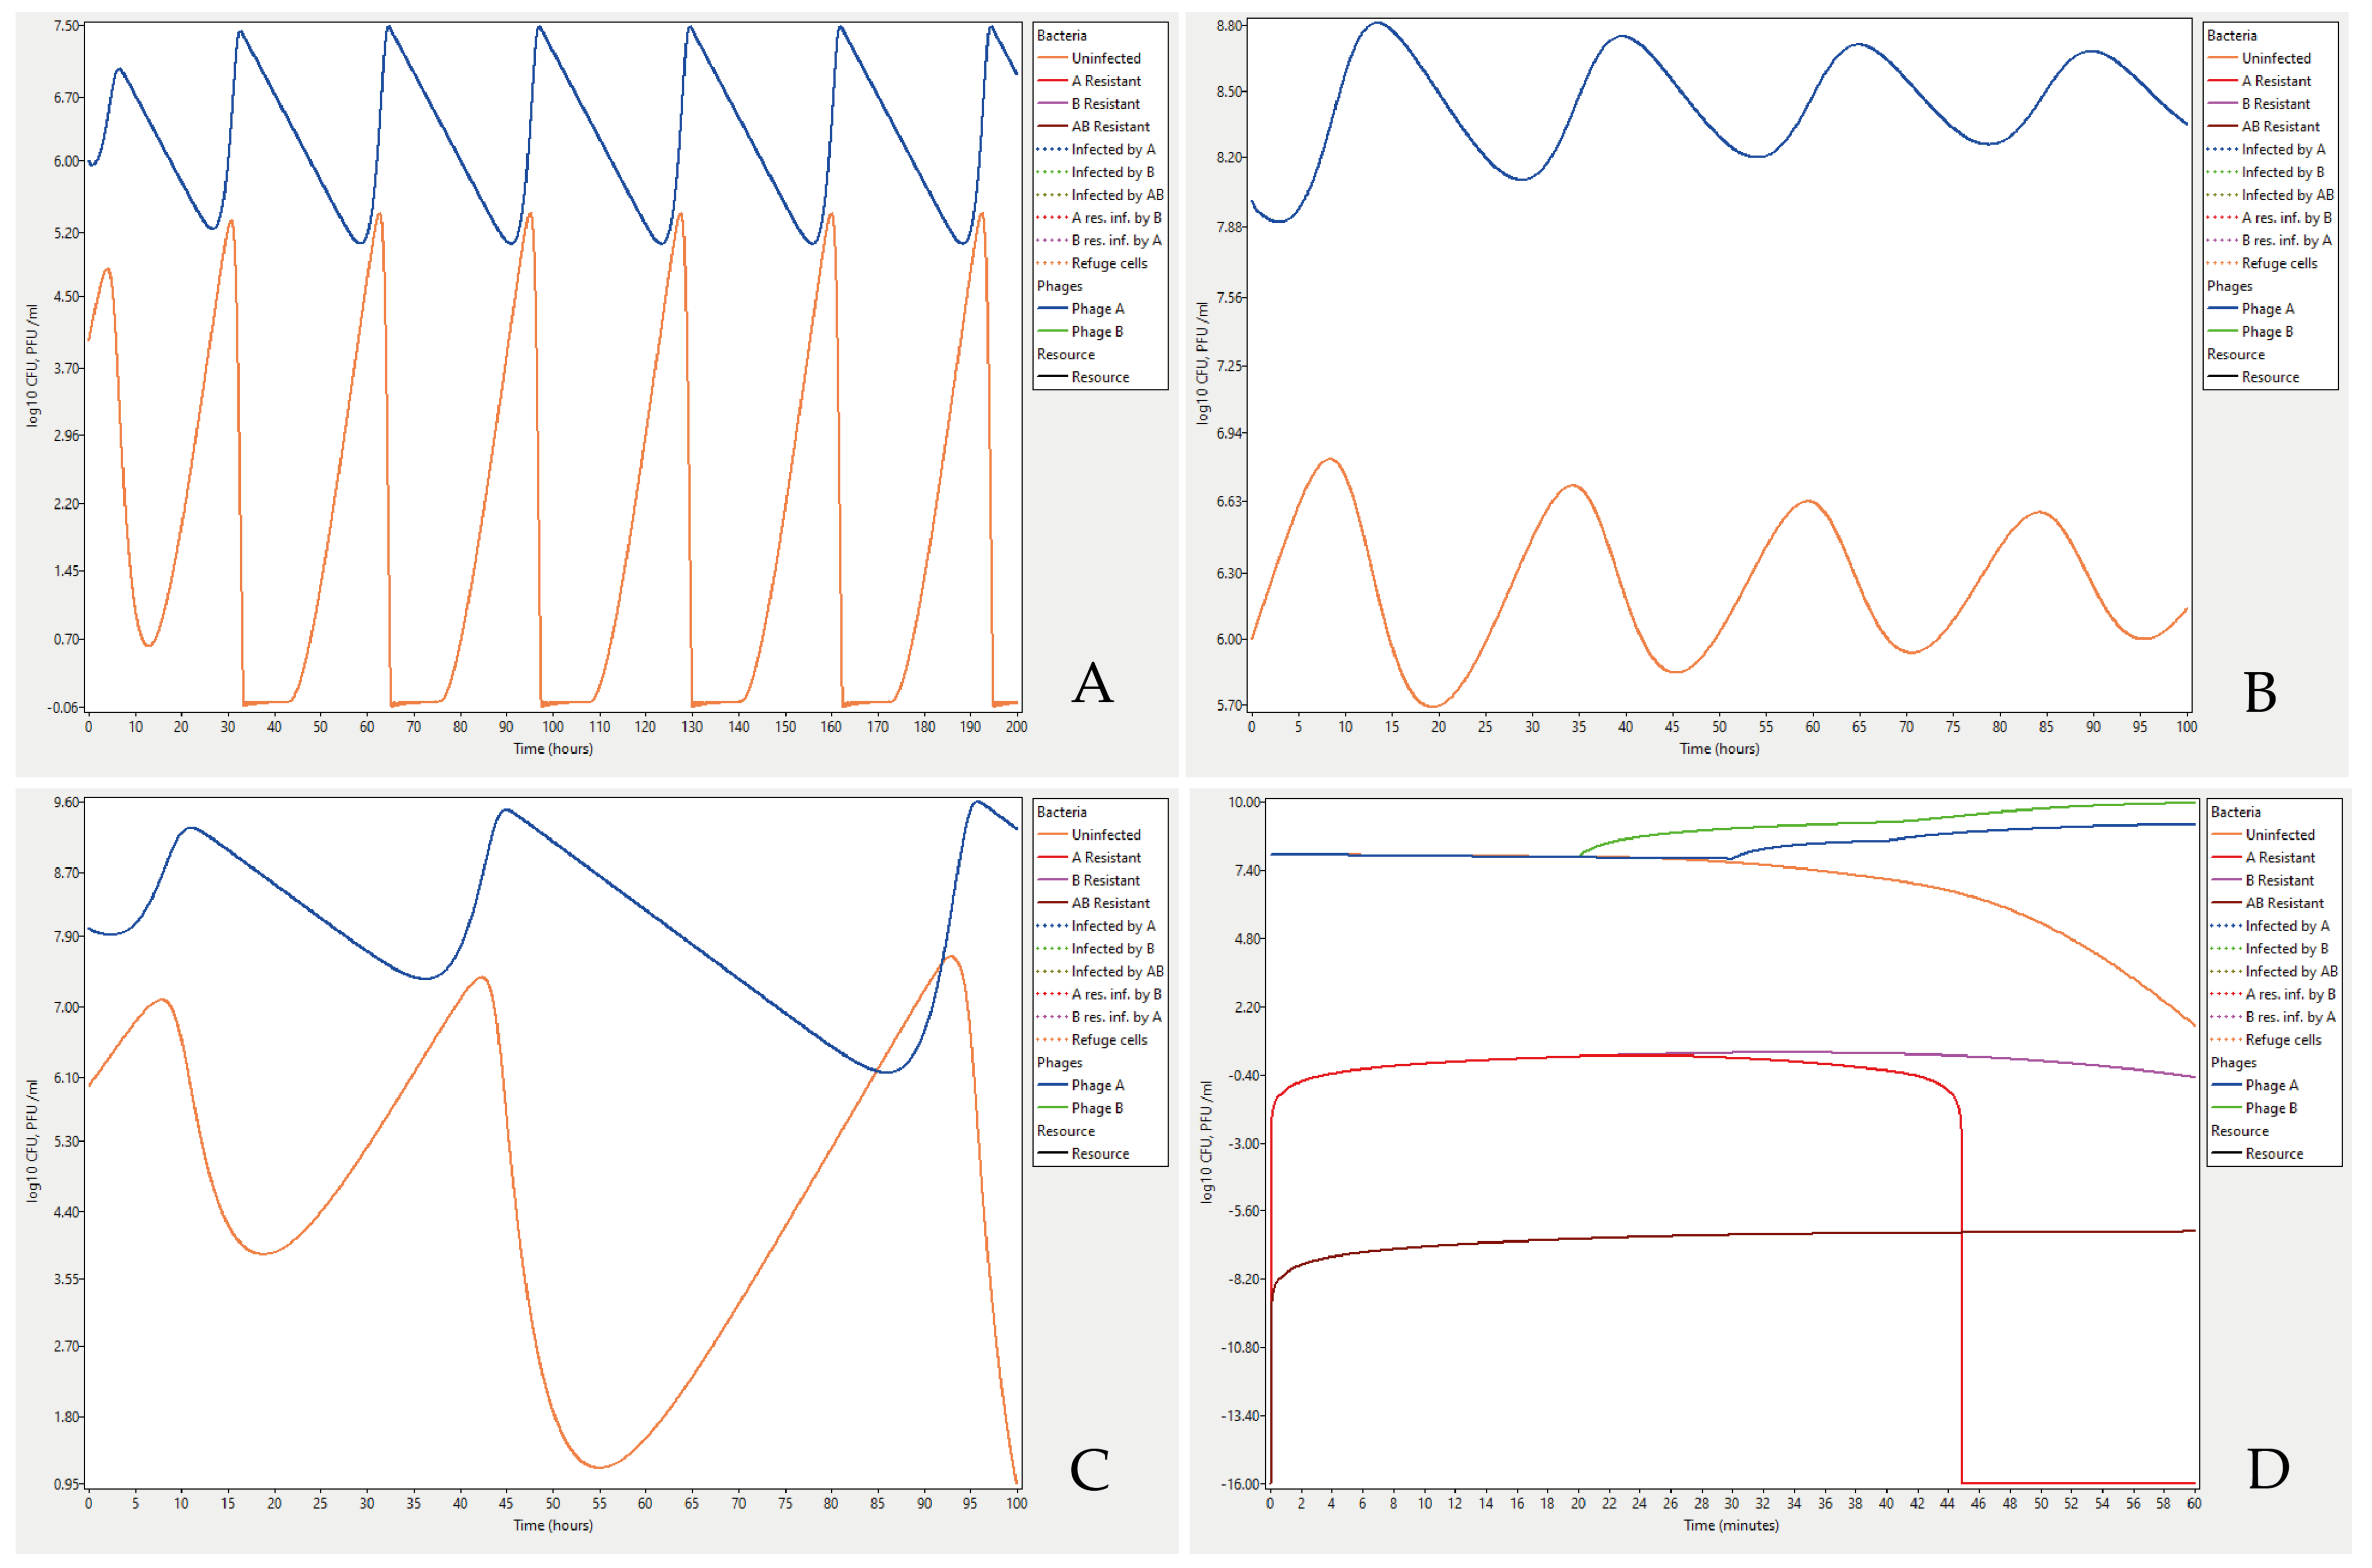
\includegraphics[width=\linewidth]{Plots/Sourced/cocktail_plot.png}
        \caption{
            Figure A) \textit{E. coli} infected with phage T4 in a chemostat exhibiting an oscillating growth behavior, following the model of \citet{bohannanEffectResourceEnrichment1997}. 
            Figure B) Oscillations of bacteria and phages can exist at higher titers, dependent on low resource concentration, following the model of \citet{lenskiDynamicsInteractionsBacteria1988}. 
            Figure C) As the concentration of resources change, this results in increasing oscillations, but not going extinct. 
            Figure D) A system modelling the interactions with phage A and B. 
        }
        \label{fig:sourced:cocktail_plot}
    \end{subfigure}
    \hfill
    \begin{subfigure}{0.49\linewidth}
        \centering
        \captionsetup{width=1\linewidth}
        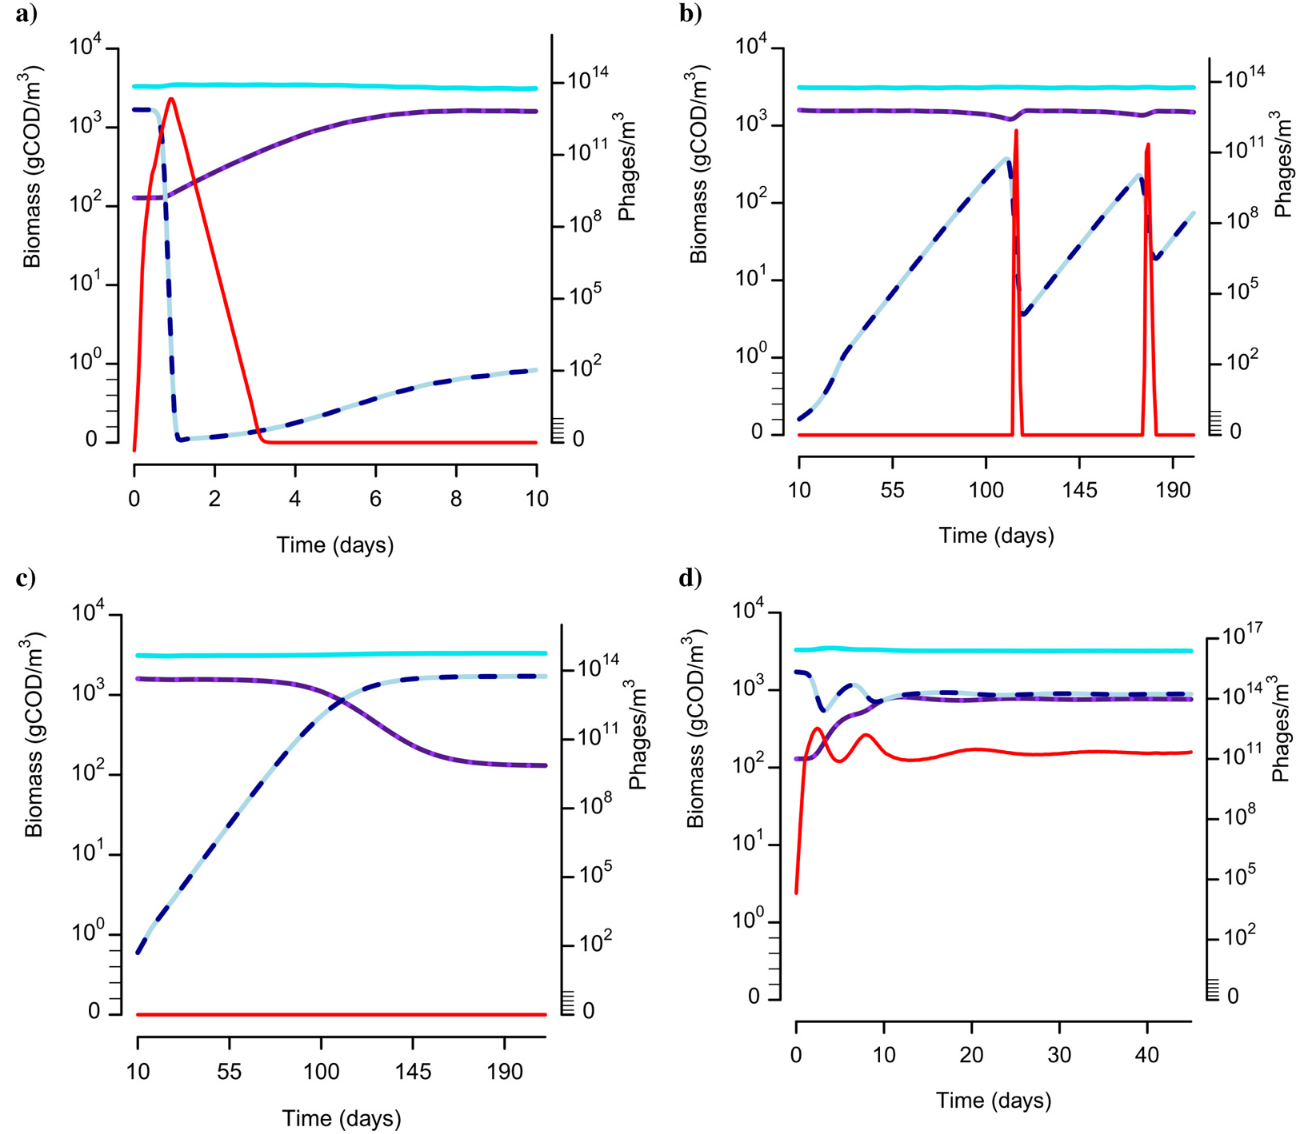
\includegraphics[width=\linewidth]{Plots/Sourced/phagedyn_plot.png}
        \caption{
            \textcolor[HTML]{551A8C}{\textbf{Purple}} is heterotrophic biomass, 
            \textcolor[HTML]{4580B4}{\textbf{Blue}} is foaming biomass, 
            \textcolor[HTML]{FF0000}{\textbf{Red}} is phages, 
            \textcolor[HTML]{01E6EE}{\textbf{Light Blue}} is total suspended solids. 
            Figure A) Biomass concentration immediately post phage dosing. 
            Figure B) Biomass concentration with low phage concentration and maintain low concentration post spike in population count. 
            Figure C) Biomass concentration when phages are extinct. 
            Figure D) Biomass concentration with a less virulent and low adsorption rate phage, co-existence with biomass reached. 
            A change in phage concentration shows a decrease in heterotrophic and foaming biomass \cite{krysiak-baltynSimulationPhageDynamics2017}. 
        }
        \label{fig:sourced:phagedyn_plot}
    \end{subfigure}
    \caption{Example output from Cocktail and PhageDyn respectively. For PhageDyn, concentration of heterotrophic biomass in an aerobic plug flow across four situations.
        See \citet{nilssonCocktailComputerProgram2022} and \citet{krysiak-baltynSimulationPhageDynamics2017} for more information on parameter values and supplementary resources. 
    }
    \label{fig:sourced:cocktail_and_phagedyn}
\end{figure}